% Cadence — The Theory of Everything (highschooler-friendly explainer)
% ENGF0031 Scenario 2 "Smart Clothing" — Parkinson's closed-loop gait garment.
% Build:  tectonic cadence_theory.tex   (XeTeX engine, auto-downloads packages)
\documentclass[11pt]{article}

% ── Fonts (XeTeX / tectonic uses system fonts directly) ──────────────────────
\usepackage{fontspec}
\setmainfont{Helvetica Neue}
\setmonofont{Menlo}[Scale=0.88]

% ── Page geometry ────────────────────────────────────────────────────────────
\usepackage[a4paper, margin=1.9cm, top=1.7cm, bottom=1.8cm]{geometry}
\usepackage{microtype}
\usepackage{amsmath}
\usepackage{graphicx}
\usepackage{booktabs}
\usepackage{enumitem}
\setlist{leftmargin=1.4em, itemsep=2pt, topsep=3pt}
\usepackage[most]{tcolorbox}
\usepackage{tikz}
\usetikzlibrary{positioning, arrows.meta, shapes.geometric, calc, fit,
                backgrounds, decorations.pathreplacing}
\usepackage{titlesec}
\usepackage{fancyhdr}

% ── Colour palette ───────────────────────────────────────────────────────────
\definecolor{teal}{HTML}{0E7C7B}
\definecolor{tealbg}{HTML}{E7F2F1}
\definecolor{amber}{HTML}{C9760D}
\definecolor{amberbg}{HTML}{FBEFDB}
\definecolor{ink}{HTML}{21302F}
\definecolor{muted}{HTML}{6B7B7A}
\definecolor{good}{HTML}{2E7D32}
\definecolor{bad}{HTML}{C0392B}
\definecolor{still}{HTML}{B9C3C3}
\definecolor{walkc}{HTML}{7FC2C0}
\definecolor{freezec}{HTML}{EBB261}
\color{ink}

% ── Section styling ──────────────────────────────────────────────────────────
\titleformat{\section}
  {\Large\bfseries\color{teal}}{\makebox[1.1em][l]{\thesection}}{0pt}{}
\titleformat{\subsection}
  {\large\bfseries\color{ink}}{}{0pt}{}
\titlespacing*{\section}{0pt}{14pt}{6pt}
\titlespacing*{\subsection}{0pt}{9pt}{3pt}

% ── Footer ───────────────────────────────────────────────────────────────────
\pagestyle{fancy}\fancyhf{}
\renewcommand{\headrulewidth}{0pt}
\renewcommand{\footrulewidth}{0.4pt}
\fancyfoot[L]{\footnotesize\color{muted}Cadence — Theory of Everything}
\fancyfoot[R]{\footnotesize\color{muted}\thepage}

% ── Callout boxes ────────────────────────────────────────────────────────────
\newtcolorbox{plain}{
  enhanced, breakable, colback=tealbg, frame hidden,
  borderline west={3pt}{0pt}{teal}, arc=2pt,
  left=10pt, right=10pt, top=7pt, bottom=7pt,
  before skip=7pt, after skip=7pt,
  fontupper=\normalsize}

\newtcolorbox{keyidea}{
  enhanced, breakable, colback=amberbg, frame hidden,
  borderline west={3pt}{0pt}{amber}, arc=2pt,
  left=10pt, right=10pt, top=7pt, bottom=7pt,
  before skip=7pt, after skip=7pt}

\newtcolorbox{fixcard}[1]{
  enhanced, breakable, colback=white, colframe=teal!70,
  boxrule=0.8pt, arc=2.5pt,
  fonttitle=\bfseries\color{white}, colbacktitle=teal,
  attach boxed title to top left={xshift=8pt, yshift=-\tcboxedtitleheight/2},
  boxed title style={colback=teal, arc=2pt},
  title={#1},
  left=9pt, right=9pt, top=9pt, bottom=8pt,
  before skip=9pt, after skip=9pt}

% little inline "plain English" lead-in
\newcommand{\pe}{\textbf{\color{teal}In plain English:}\ }

% TikZ shared styles
\tikzset{
  blok/.style={rounded corners=3pt, draw=teal, line width=1pt, fill=tealbg,
               align=center, font=\small, inner sep=5pt},
  flow/.style={-{Latex[length=2.6mm]}, line width=1pt, draw=teal},
  flowA/.style={-{Latex[length=2.6mm]}, line width=1pt, draw=amber},
  dia/.style={diamond, aspect=2.1, draw=amber, line width=1pt, fill=amberbg,
              align=center, font=\small, inner sep=1pt},
}

\begin{document}

% ════════════════════════════════════════════════════════════════════════════
% TITLE BLOCK
% ════════════════════════════════════════════════════════════════════════════
\begin{tcolorbox}[enhanced, colback=teal, colframe=teal, arc=4pt,
  left=16pt, right=16pt, top=13pt, bottom=13pt, boxrule=0pt]
  {\color{white}\Huge\bfseries Cadence: The Theory of Everything}\\[5pt]
  {\color{white}\large How our smart anklet spots a Parkinson's ``freeze'' and
   buzzes you free \,---\, explained from scratch.}\\[8pt]
  {\color{tealbg}\footnotesize ENGF0031 Scenario 2 \textbullet\ Smart Clothing
   \quad\textbullet\quad Every number in here is from our own real ankle
   recording \texttt{capture1.csv}.}
\end{tcolorbox}

\vspace{2pt}
\noindent\small This guide explains \emph{everything} the project does and
\emph{why}, in plain language, with pictures. The last section is the honest
``things that broke and how we fixed them'' diary. No prior physics needed.
\normalsize

% ════════════════════════════════════════════════════════════════════════════
\section{The big idea: a thermostat for your feet}

People with Parkinson's disease sometimes get \textbf{freezing of gait (FoG)}:
their feet feel ``glued'' to the floor even though they want to walk. It is a
major cause of falls. A weird but well-proven trick helps: give the person a
\textbf{steady external beat} --- a metronome tick, a line on the floor, or a
gentle buzz --- and their brain ``borrows'' that rhythm and starts stepping
again. This is called \emph{rhythmic cueing}.

Our garment, \textbf{Cadence}, is a small computer worn on the ankle that does
this automatically. It watches how your leg is moving, decides when you have
frozen, and buzzes a beat \emph{only then}. When you start walking again, it
goes quiet. That ``watch $\rightarrow$ decide $\rightarrow$ act $\rightarrow$
watch again'' circle is called a \textbf{closed loop}.

\begin{plain}
\pe It is a thermostat, but for walking. A thermostat senses the temperature
and flips the heater on only when the room gets cold. Cadence senses your
\emph{leg}, and flips a \emph{buzzer} on only when your walking ``freezes''.
\end{plain}

\begin{center}
\resizebox{0.99\linewidth}{!}{%
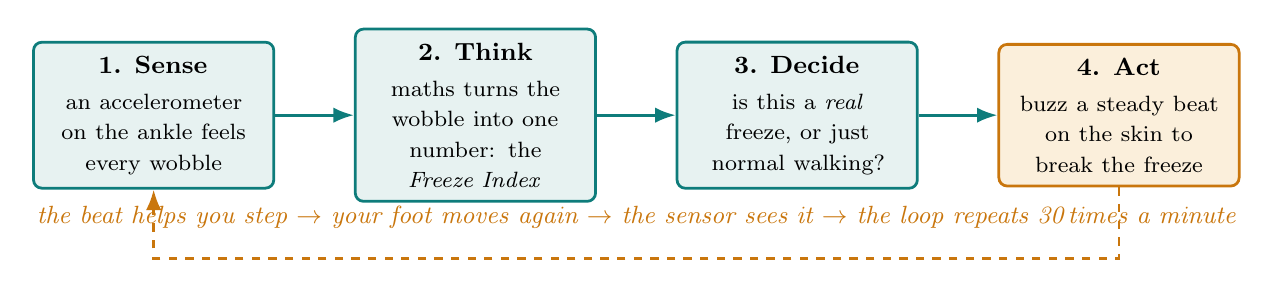
\begin{tikzpicture}[node distance=10mm]
  \node[blok, text width=27mm] (s) {\textbf{1. Sense}\\[2pt]\footnotesize
        an accelerometer on the ankle feels every wobble};
  \node[blok, text width=27mm, right=of s] (b) {\textbf{2. Think}\\[2pt]\footnotesize
        maths turns the wobble into one number: the \emph{Freeze Index}};
  \node[blok, text width=27mm, right=of b] (d) {\textbf{3. Decide}\\[2pt]\footnotesize
        is this a \emph{real} freeze, or just normal walking?};
  \node[blok, text width=27mm, right=of d, fill=amberbg, draw=amber] (c)
        {\textbf{4. Act}\\[2pt]\footnotesize buzz a steady beat on the skin to
         break the freeze};
  \draw[flow] (s) -- (b);
  \draw[flow] (b) -- (d);
  \draw[flow] (d) -- (c);
  % feedback loop
  \draw[flowA, dashed] (c.south) -- ++(0,-9mm) coordinate(low)
        -| (s.south);
  \node[font=\itshape\small, text=amber, align=center] at ([yshift=-13mm]$(s)!0.5!(c)$)
        {the beat helps you step $\rightarrow$ your foot moves again $\rightarrow$ the sensor sees it $\rightarrow$ the loop repeats 30\,times a minute};
\end{tikzpicture}}
\end{center}

% ════════════════════════════════════════════════════════════════════════════
\section{Step 1 --- Feeling movement: the accelerometer}

The sensor is an \textbf{accelerometer}: imagine a tiny weight on tiny springs
inside the chip. When the chip speeds up, slows down, or tilts, the weight lags
and the springs stretch, and the chip measures that stretch. It reports three
numbers --- one for each direction in space: $x$ (side to side), $y$ (up and
down), $z$ (forward and back). Gravity always tugs the weight ``down'', so even
when you are still the sensor reads about \textbf{1\,g} (one gravity) pointing
at the floor.

We sample these three numbers \textbf{64 times every second} (64\,Hz). That is
fast enough to see a leg tremble but slow enough for a coin-cell-powered chip.

\begin{center}
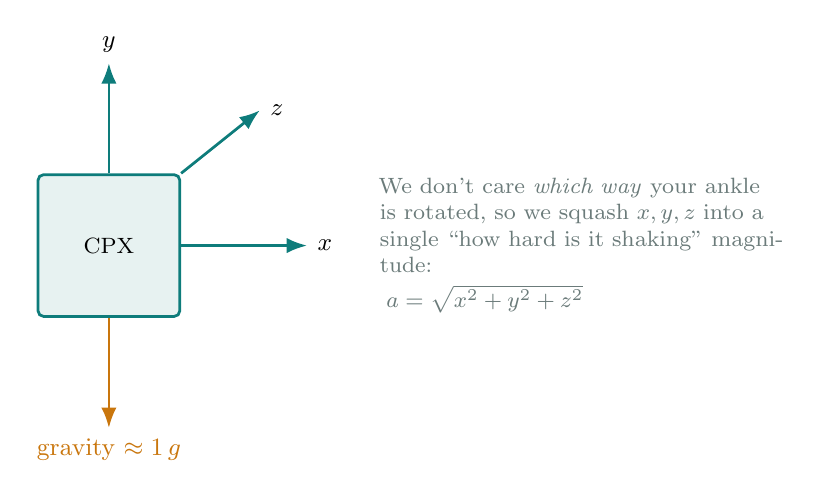
\begin{tikzpicture}[scale=1]
  % the board
  \node[draw=teal, line width=1pt, fill=tealbg, rounded corners=2pt,
        minimum width=18mm, minimum height=18mm, font=\footnotesize] (cpx) {CPX};
  % axes
  \draw[flow] (cpx.east) -- ++(1.6,0) node[right, font=\small]{$x$};
  \draw[flow] (cpx.north) -- ++(0,1.4) node[above, font=\small]{$y$};
  \draw[flow] (cpx.north east) -- ++(1.0,0.8) node[right, font=\small]{$z$};
  % gravity
  \draw[flowA] (cpx.south) -- ++(0,-1.4) node[below, font=\small, text=amber]{gravity $\approx 1\,g$};
  \node[align=left, font=\footnotesize, text=muted, right=24mm of cpx, text width=52mm]
    {We don't care \emph{which way} your ankle is rotated, so we squash $x,y,z$
     into a single ``how hard is it shaking'' magnitude:
     \\[3pt]
     \centering$\;a=\sqrt{x^{2}+y^{2}+z^{2}}\;$};
\end{tikzpicture}
\end{center}

\begin{plain}
\pe Strap the chip to your ankle however you like --- we only use the
\emph{total} shake $a=\sqrt{x^2+y^2+z^2}$, so it works no matter how the strap is
twisted. That trick is called being \emph{orientation-invariant}.
\end{plain}

% ════════════════════════════════════════════════════════════════════════════
\section{Step 2 --- The magic number: frequency and the Freeze Index}

Here is the key insight the whole project rests on. \textbf{Walking and freezing
shake your leg at different \emph{speeds of wiggle}.}

\begin{itemize}
  \item \textbf{Walking} is a slow, big swing --- about 1 to 2 steps per second.
        We call that a low \emph{frequency} (0.5--3\,Hz), the ``walking band''.
  \item \textbf{Freezing} is a fast, small \emph{tremble} --- the leg vibrates
        roughly 3 to 8 times per second while going nowhere. That is a high
        frequency (3--8\,Hz), the ``freeze band''.
\end{itemize}

\pe Frequency just means \emph{how many wiggles per second}. Think bass notes
(slow, deep) versus treble notes (fast, high). Walking is the bass; a freeze
tremor is the treble.

To measure ``how much slow wiggle vs.\ how much fast wiggle'' is in a chunk of
signal, we use a standard maths recipe (a \emph{power spectrum}). You can picture
it as the bar-graph equaliser on a music app: it tells you how loud each
frequency is in the mix.

\begin{center}
\resizebox{0.92\linewidth}{!}{%
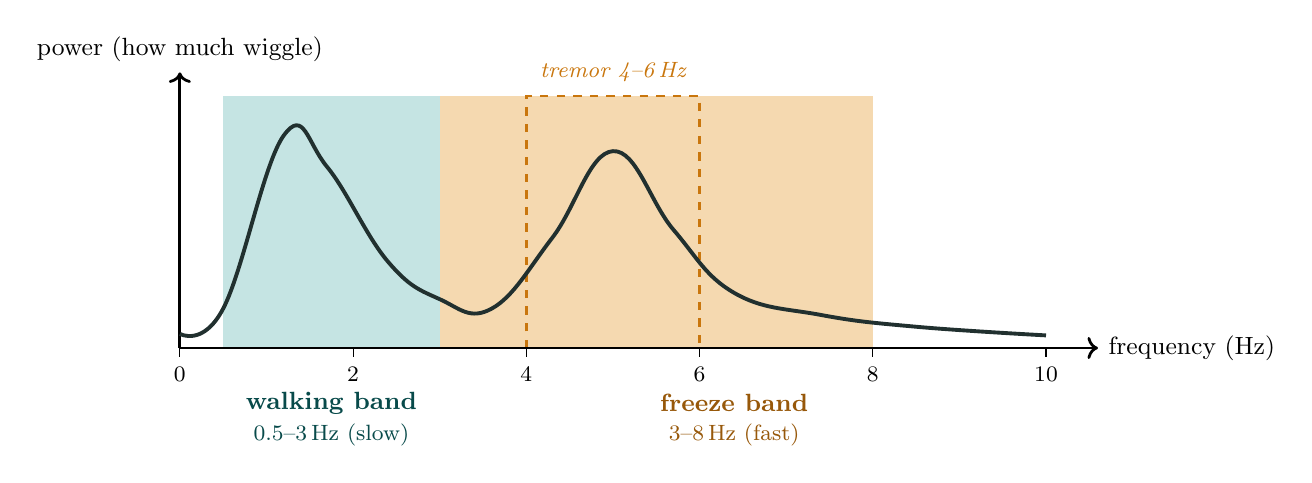
\begin{tikzpicture}[x=11mm, y=10mm]
  % bands behind
  \fill[walkc!45] (0.5,0) rectangle (3,3.2);
  \fill[freezec!50] (3,0) rectangle (8,3.2);
  % tremor sub-band outline
  \draw[amber, dashed, line width=0.9pt] (4,0) rectangle (6,3.2);
  % axes
  \draw[->, line width=1pt] (0,0) -- (10.6,0) node[right, font=\small]{frequency (Hz)};
  \draw[->, line width=1pt] (0,0) -- (0,3.5) node[above, font=\small]{power (how much wiggle)};
  \foreach \xx in {0,2,4,6,8,10} \draw (\xx,0) -- (\xx,-0.12) node[below, font=\footnotesize]{\xx};
  % the spectrum curve (illustrative shape)
  \draw[line width=1.4pt, ink] plot[smooth, tension=0.7] coordinates
    {(0,0.18)(0.5,0.5)(1.2,2.7)(1.7,2.3)(2.4,1.1)(3,0.62)
     (3.6,0.5)(4.3,1.4)(5,2.5)(5.7,1.5)(6.4,0.7)(7.4,0.42)(8.5,0.27)(10,0.16)};
  % labels
  \node[font=\small\bfseries, text=teal!60!black] at (1.75,-0.7) {walking band};
  \node[font=\footnotesize, text=teal!60!black] at (1.75,-1.1) {0.5--3\,Hz (slow)};
  \node[font=\small\bfseries, text=amber!75!black] at (6.4,-0.7) {freeze band};
  \node[font=\footnotesize, text=amber!75!black] at (6.4,-1.1) {3--8\,Hz (fast)};
  \node[font=\footnotesize\itshape, text=amber] at (5,3.5) {tremor 4--6\,Hz};
\end{tikzpicture}}
\\[2pt]
{\footnotesize\color{muted}(Illustrative shape of a spectrum. Walking puts a big
bump in the slow band; a freeze adds a bump in the fast band.)}
\end{center}

Now the clever bit. \textbf{Moore et al.\ (2008)} defined the \textbf{Freeze
Index (FI)} as a simple ratio:

\begin{center}
\begin{tcolorbox}[enhanced, colback=white, colframe=teal, boxrule=1pt, arc=3pt,
   width=0.86\linewidth, halign=center, top=8pt, bottom=8pt]
  \large$\displaystyle
  \text{Freeze Index}=\frac{\text{power in the FAST freeze band (3--8\,Hz)}}
                            {\text{power in the SLOW walking band (0.5--3\,Hz)}}$
\end{tcolorbox}
\end{center}

\begin{itemize}
  \item \textbf{Walking:} lots of slow power, little fast power
        $\Rightarrow$ \emph{small} FI (a small number on top divided by a big
        number on the bottom).
  \item \textbf{Freezing:} the leg trembles fast but doesn't travel, so fast
        power shoots up and slow power collapses $\Rightarrow$ \emph{big} FI.
\end{itemize}

\begin{keyidea}
\textbf{One number tells the whole story.} A low Freeze Index means ``moving
normally''. A high Freeze Index means ``shaking in place'' --- the signature of a
freeze. Everything after this is just deciding \emph{how high is high enough}.
\end{keyidea}

% ════════════════════════════════════════════════════════════════════════════
\section{Step 3 --- Chopping time into windows}

We can't compute a frequency from a single instant --- you need to watch the leg
for a little while to see how fast it's wiggling. So we slice the stream into
\textbf{4-second windows}, and we slide the window along by \textbf{2 seconds}
each time, so windows overlap by half. That gives us a fresh decision
\textbf{every 2 seconds} while still having 4 seconds of context to measure
frequency accurately.

\pe Like reading a sentence with a 4-word-wide highlighter that you shuffle
forward 2 words at a time --- you always see enough words to understand, and you
re-read often enough to keep up.

\begin{center}
\resizebox{0.99\linewidth}{!}{%
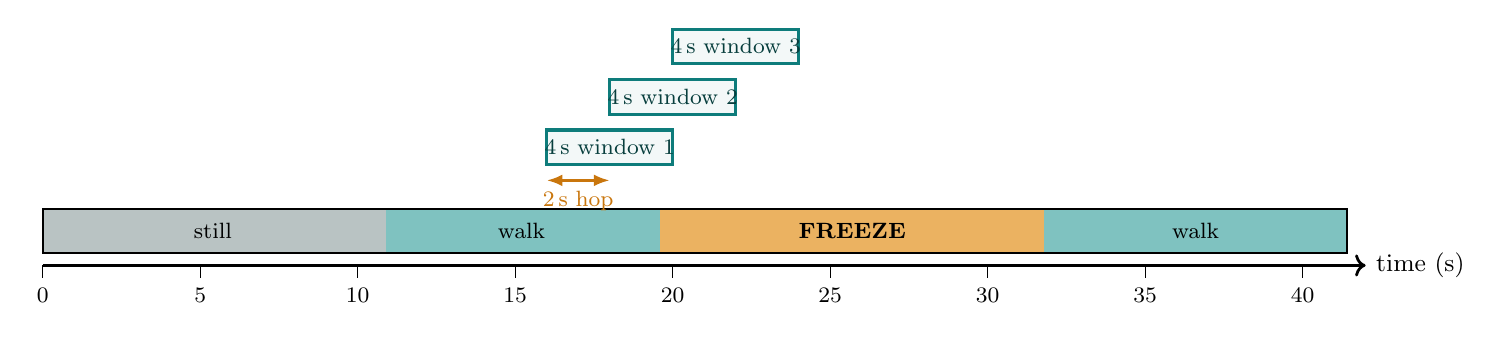
\begin{tikzpicture}[x=4.0mm, y=8mm]
  % phase strip (real boundaries: still 0-10.9, walk 10.9-19.6, freeze 19.6-31.8, walk 31.8-41.4)
  \fill[still]   (0,0)    rectangle (10.9,0.7);
  \fill[walkc]   (10.9,0) rectangle (19.6,0.7);
  \fill[freezec] (19.6,0) rectangle (31.8,0.7);
  \fill[walkc]   (31.8,0) rectangle (41.4,0.7);
  \draw[line width=0.8pt] (0,0) rectangle (41.4,0.7);
  \node[font=\footnotesize] at (5.4,0.35){still};
  \node[font=\footnotesize] at (15.2,0.35){walk};
  \node[font=\footnotesize\bfseries] at (25.7,0.35){FREEZE};
  \node[font=\footnotesize] at (36.6,0.35){walk};
  % time axis
  \draw[->,line width=1pt] (0,-0.2) -- (42,-0.2) node[right,font=\small]{time (s)};
  \foreach \tt in {0,5,...,40} \draw (\tt,-0.2)--(\tt,-0.4) node[below,font=\footnotesize]{\tt};
  % three overlapping windows above the strip
  \foreach \start/\lab/\yy in {16/1/1.4, 18/2/2.2, 20/3/3.0}{
    \draw[teal, line width=1.1pt, fill=tealbg, fill opacity=0.5]
        (\start,\yy) rectangle (\start+4,\yy+0.55);
    \node[font=\footnotesize, text=teal!50!black] at (\start+2,\yy+0.28){4\,s window \lab};
  }
  \draw[{Latex[length=2mm]}-{Latex[length=2mm]}, amber, line width=1pt]
        (16,1.15) -- (18,1.15) node[midway, below, font=\footnotesize, text=amber]{2\,s hop};
\end{tikzpicture}}
\\[2pt]
{\footnotesize\color{muted}(The coloured strip is our real recording. The
overlapping boxes are the sliding analysis windows.)}
\end{center}

% ════════════════════════════════════════════════════════════════════════════
\section{Step 4 --- The decision, with two safety nets}

A naive detector would just say ``Freeze Index above some line $\Rightarrow$
buzz''. But that buzzes at the wrong times. Two famous failure modes, and how we
block each one:

\subsection{The threshold: where is ``the line''?}
From our real recording, normal \textbf{walking} peaked at a Freeze Index of
\textbf{2.08}. A real \textbf{freeze} hit \textbf{6.6, 21.4, 5.3}\dots\ far
higher. So we set the line at \textbf{FI $>$ 2.10} --- just above the worst
walking value, so ordinary walking can never trip it. (The textbook starting
point is 2.0; we \emph{tuned} ours to 2.10 to fit our own data.)

\subsection{Safety net \#1 --- the energy gate (don't shout at a resting leg)}
A ratio can be misleading. If the leg is \emph{completely still}, both bands are
just tiny sensor noise --- and noise over noise can randomly look ``high''. So
before we even look at the Freeze Index we ask: \textbf{is the leg actually doing
anything?} We add up the real movement power; if it is below
\textbf{ENERGY\_FLOOR = 300} (a resting ankle reads only $\sim$130--270), we
declare ``not moving'' and stay silent no matter what the ratio says.

\subsection{Safety net \#2 --- debounce \& hysteresis (don't trust one blip)}
A single noisy window shouldn't fire the motor. So we \emph{debounce}: the buzzer
only switches \textbf{ON after 2 freeze-windows in a row}, and only switches
\textbf{OFF after 2 clear windows in a row}. Requiring a run before changing
state is called \emph{hysteresis}.

\pe Like waiting to feel a second raindrop before opening your umbrella --- and
leaving it open until you're sure the rain has really stopped.

\begin{center}
\resizebox{0.80\linewidth}{!}{%
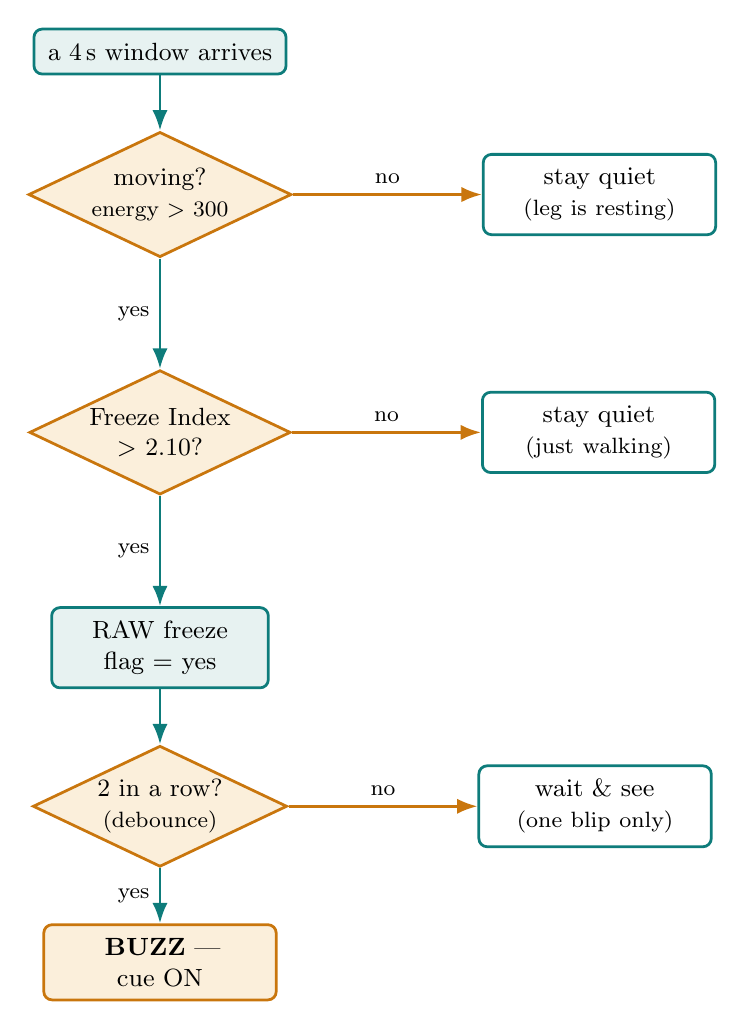
\begin{tikzpicture}[node distance=7mm and 14mm]
  \node[blok] (start) {a 4\,s window arrives};
  \node[dia, below=of start] (mov) {moving?\\\footnotesize energy $>$ 300};
  \node[dia, below=14mm of mov] (fi) {Freeze Index\\$>$ 2.10?};
  \node[blok, below=14mm of fi, text width=24mm] (raw) {RAW freeze flag = yes};
  \node[dia, below=of raw] (deb) {2 in a row?\\\footnotesize (debounce)};
  \node[blok, fill=amberbg, draw=amber, below=of deb, text width=26mm] (buzz)
        {\textbf{BUZZ} --- cue ON};
  % quiet sinks on the right
  \node[blok, right=24mm of mov, fill=white, text width=26mm] (q1){stay quiet\\\footnotesize (leg is resting)};
  \node[blok, right=24mm of fi, fill=white, text width=26mm] (q2){stay quiet\\\footnotesize (just walking)};
  \node[blok, right=24mm of deb, fill=white, text width=26mm] (q3){wait \& see\\\footnotesize (one blip only)};
  \draw[flow] (start)--(mov);
  \draw[flow] (mov)-- node[left,font=\footnotesize]{yes} (fi);
  \draw[flow] (fi)-- node[left,font=\footnotesize]{yes} (raw);
  \draw[flow] (raw)--(deb);
  \draw[flow] (deb)-- node[left,font=\footnotesize]{yes} (buzz);
  \draw[flowA] (mov)-- node[above,font=\footnotesize]{no} (q1);
  \draw[flowA] (fi)-- node[above,font=\footnotesize]{no} (q2);
  \draw[flowA] (deb)-- node[above,font=\footnotesize]{no} (q3);
\end{tikzpicture}}
\end{center}

\subsection*{Watching the safety nets work, second by second}
Here is the actual run over our recording. Row~1 is the raw ``this window is over
the line'' flag; Row~2 is what the motor actually does after debouncing.

\begin{center}
\resizebox{0.99\linewidth}{!}{%
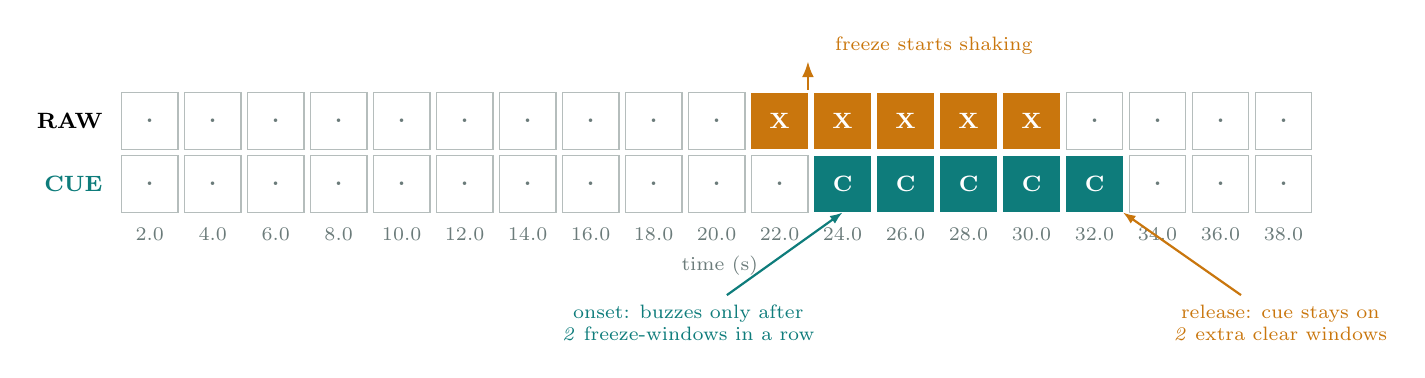
\begin{tikzpicture}[x=8mm, y=8mm]
  % 19 windows, t = 2..38. raw freeze at i10..i14 ; cue at i11..i15
  \foreach \i in {0,...,18}{
    \pgfmathsetmacro\tlab{2+2*\i}
    % raw row (y=1)
    \pgfmathparse{(\i>=10 && \i<=14)?1:0}\ifnum\pgfmathresult=1
      \fill[amber] (\i,1) rectangle (\i+0.9,1.9);
      \node[white,font=\footnotesize\bfseries] at (\i+0.45,1.45){X};
    \else
      \draw[muted!50] (\i,1) rectangle (\i+0.9,1.9);
      \node[muted,font=\footnotesize] at (\i+0.45,1.45){\textbf{.}};
    \fi
    % cue row (y=0)
    \pgfmathparse{(\i>=11 && \i<=15)?1:0}\ifnum\pgfmathresult=1
      \fill[teal] (\i,0) rectangle (\i+0.9,0.9);
      \node[white,font=\footnotesize\bfseries] at (\i+0.45,0.45){C};
    \else
      \draw[muted!50] (\i,0) rectangle (\i+0.9,0.9);
      \node[muted,font=\footnotesize] at (\i+0.45,0.45){\textbf{.}};
    \fi
    \node[font=\scriptsize, text=muted] at (\i+0.45,-0.35){\tlab};
  }
  \node[left, font=\footnotesize\bfseries] at (0,1.45){RAW\ \ };
  \node[left, font=\footnotesize\bfseries, text=teal] at (0,0.45){CUE\ \ };
  \node[font=\scriptsize, text=muted] at (9.5,-0.85){time (s)};
  % annotations
  \draw[{Latex[length=2mm]}-, amber, line width=0.9pt] (10.9,2.4) -- ++(0,-0.45);
  \node[font=\scriptsize, text=amber, align=center] at (12.9,2.65){freeze starts shaking};
  \node[font=\scriptsize, text=teal, align=center] (a2) at (9.0,-1.75)
       {onset: buzzes only after\\\emph{2} freeze-windows in a row};
  \draw[{Latex[length=1.6mm]}-, teal, line width=0.8pt] (11.45,0.0) -- (a2);
  \node[font=\scriptsize, text=amber, align=center] (a3) at (18.4,-1.75)
       {release: cue stays on\\\emph{2} extra clear windows};
  \draw[{Latex[length=1.6mm]}-, amber, line width=0.8pt] (15.9,0.0) -- (a3);
\end{tikzpicture}}
\end{center}

\noindent Notice three things: (1)~the cue starts \emph{one window later} than
the raw flag --- that is the 2-in-a-row onset rule; (2)~it \emph{stays on} for one
window after the shaking stops --- the 2-clear release rule, so it doesn't flicker;
(3)~the very first freeze window (t\,=\,20\,s) didn't even raise the raw flag,
because that window straddles the walk$\to$freeze boundary and is half-walking.
We catch the freeze 2\,s later anyway.

% ════════════════════════════════════════════════════════════════════════════
\section{Step 5 --- Did it actually work? The real scoreboard}

We recorded one continuous $\sim$41-second trip on a real ankle:
\textbf{still $\rightarrow$ walk $\rightarrow$ freeze $\rightarrow$ walk}. Here is
the real trace the detector saw (top: how hard the ankle shook; bottom: the
Freeze Index, with our 2.10 line):

\begin{center}
  
\includegraphics[width=0.98\linewidth]{figs/capture1_trace.pdf}
\end{center}

To grade it we compare, window by window, what the detector said against the
truth. Four outcomes are possible, shown in a \textbf{confusion matrix}:

\begin{center}
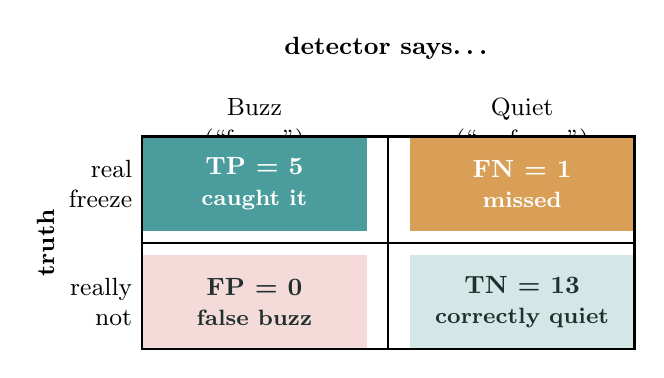
\begin{tikzpicture}[x=34mm, y=15mm]
  % headers
  \node[font=\small\bfseries] at (0.5,2.15){\textsc{detector says\dots}};
  \node[font=\small, align=center] at (0,1.5){Buzz\\\footnotesize (``freeze'')};
  \node[font=\small, align=center] at (1,1.5){Quiet\\\footnotesize (``no freeze'')};
  \node[font=\small\bfseries, rotate=90, align=center] at (-0.78,0.5){\textsc{truth}};
  \node[font=\small, align=right, anchor=east] at (-0.42,1){real\\freeze};
  \node[font=\small, align=right, anchor=east] at (-0.42,0){really\\not};
  % cells
  \fill[teal!75]   (-0.42,0.6) rectangle (0.42,1.4);
  \node[white,font=\bfseries\small,align=center] at (0,1){TP = 5\\\footnotesize caught it};
  \fill[amber!70]  (0.58,0.6) rectangle (1.42,1.4);
  \node[white,font=\bfseries\small,align=center] at (1,1){FN = 1\\\footnotesize missed};
  \fill[bad!18]    (-0.42,-0.4) rectangle (0.42,0.4);
  \node[ink,font=\bfseries\small,align=center] at (0,0){FP = 0\\\footnotesize false buzz};
  \fill[teal!18]   (0.58,-0.4) rectangle (1.42,0.4);
  \node[ink,font=\bfseries\small,align=center] at (1,0){TN = 13\\\footnotesize correctly quiet};
  \draw[line width=0.8pt] (-0.42,-0.4) rectangle (1.42,1.4);
  \draw[line width=0.8pt] (0.5,-0.4)--(0.5,1.4);
  \draw[line width=0.8pt] (-0.42,0.5)--(1.42,0.5);
\end{tikzpicture}
\end{center}

\begin{tcolorbox}[enhanced, colback=tealbg, colframe=teal, boxrule=1pt, arc=3pt,
   left=12pt, right=12pt, top=8pt, bottom=8pt]
\textbf{The two headline numbers (this is what the worksheet grades --- not
``accuracy''):}
\begin{itemize}
  \item \textbf{Sensitivity} $=\dfrac{\text{TP}}{\text{TP}+\text{FN}}
        =\dfrac{5}{6}=\mathbf{83\%}$ \;---\; ``of all the real freezes, how many
        did we \emph{catch}?'' (Don't leave the patient stuck.)
  \item \textbf{Specificity} $=\dfrac{\text{TN}}{\text{TN}+\text{FP}}
        =\dfrac{13}{13}=\mathbf{100\%}$ \;---\; ``of all the non-freezes, how many
        did we correctly \emph{leave alone}?'' (Don't annoy them with wrong buzzes.)
\end{itemize}
\end{tcolorbox}

\subsection*{Why not just say ``accuracy''?}
Because freezes are \emph{rare}. In a long walk, a lazy detector that buzzes
\emph{never} would still be ``correct'' most of the time --- high accuracy, but
totally useless (it catches zero freezes). Splitting the score into
\textbf{sensitivity} (catch rate) and \textbf{specificity} (leave-alone rate)
exposes that trick and is the honest way to report a medical detector. Our one
miss (FN) is the very first 2-second slice of the freeze, which the next window
catches --- so the wearer is still cued, just $\sim$2\,s later.

% ════════════════════════════════════════════════════════════════════════════
\section{The honest part: everything that broke, and how we fixed it}

Real engineering is mostly fixing things that don't work the first time. Here is
our actual debugging diary --- the bugs, \emph{why} each happened, and the fix.

\subsection*{A. Getting the data off the board}

\begin{fixcard}{Bug 1 --- a flaky USB cable kept dropping mid-recording}
\textbf{What happened.} Half-way through a capture the serial connection died and
the script crashed, losing the run. \\
\textbf{Why.} The only cable we had was failing intermittently --- the laptop
briefly lost the board, and our code assumed the connection never disappears. \\
\textbf{The fix.} We made the reader \emph{reconnect automatically}: if the port
vanishes it waits, re-opens it, and keeps reading. The next capture survived a
drop and still produced one clean 41-second file.
\end{fixcard}

\begin{fixcard}{Bug 2 --- we were ``flying blind'' (no live readout)}
\textbf{What happened.} While recording, nothing printed, so we couldn't tell if
data was flowing. \\
\textbf{Why.} Python \emph{buffers} its output --- it holds text back until a big
chunk piles up, instead of showing each line. \\
\textbf{The fix.} We ran Python in \emph{unbuffered} mode (the \texttt{-u} flag),
so every sample echoed instantly and we could watch the capture live.
\end{fixcard}

\subsection*{B. Tuning the brain (the parameters we ``fixed'' to real values)}

\begin{fixcard}{Bug 3 --- normal walking nearly triggered a false freeze}
\textbf{What happened.} With the textbook line at FI\,$=$\,2.0, a stride of
\emph{normal walking} hit FI\,$=$\,2.08 and almost set off the buzzer. \\
\textbf{Why.} Our walking happened to be a touch shakier than the textbook
assumed, so its Freeze Index crept above 2.0. \\
\textbf{The fix.} We \emph{tuned the threshold up to 2.10}, just above the worst
real walking value. Result: walking now \emph{never} fires (specificity 100\%),
and real freezes (FI 3--21) still sail over the line.
\end{fixcard}

\begin{fixcard}{Bug 4 --- a perfectly still leg could randomly look ``frozen''}
\textbf{What happened.} When the leg was motionless, the Freeze Index sometimes
spiked for no real reason. \\
\textbf{Why.} The Index is a \emph{ratio} of two tiny noise signals; dividing
noise by noise gives garbage that can look high. \\
\textbf{The fix.} We added the \emph{energy gate} (safety net \#1): if total
movement is below 300, declare ``not moving'' and stay silent regardless of the
ratio. A freeze is \emph{trembling while trying to move} --- a still leg can't be
freezing.
\end{fixcard}

\begin{fixcard}{Bug 5 --- single noisy windows caused jittery buzzing}
\textbf{What happened.} One odd window could flick the motor on (or off) for a
moment --- annoying and unconvincing. \\
\textbf{Why.} We were reacting to \emph{every} individual window with no memory. \\
\textbf{The fix.} We added \emph{debounce + hysteresis} (safety net \#2): need 2
freeze-windows in a row to start, and 2 clear windows in a row to stop. The cue
is now smooth and only responds to \emph{sustained} freezes.
\end{fixcard}

\begin{fixcard}{Bug 6 --- the detector ``missed'' the first freeze window (a false negative)}
\textbf{What happened.} The window centred at t\,=\,20\,s (right as the freeze
began) scored a low FI and was marked ``no freeze''. \\
\textbf{Why.} A 4-second window that lands on the walk$\to$freeze boundary is
\emph{half walking, half freezing}, so its average Freeze Index is watered down. \\
\textbf{The fix \& trade-off.} Real freezes last several seconds, so the very next
window (t\,=\,22\,s) catches it and the cue fires --- only $\sim$2\,s late, which is
clinically fine. We \emph{accept} this one miss to keep false buzzes at zero. (A
neural-net upgrade, FoGNet, is the ``given more time'' way to shave it further.)
\end{fixcard}

\subsection*{C. Building the documents (LaTeX \& shell gremlins)}

\begin{fixcard}{Bug 7 --- the worksheet PDF wouldn't compile}
\textbf{What happened.} Two LaTeX errors: a maths line with tangled
\texttt{\textbackslash(\,\dots\,\textbackslash)} and \texttt{\$\dots\$} markers,
and an ``undefined command'' for $\lVert\cdot\rVert$. \\
\textbf{Why.} The maths delimiters were mismatched, and the symbol needed the
\texttt{amsmath} package which wasn't loaded. \\
\textbf{The fix.} We rewrote the line cleanly and added
\texttt{\textbackslash usepackage\{amsmath\}}. It compiled.
\end{fixcard}

\begin{fixcard}{Bug 8 --- a code block split across two pages, and a shell glob blew up}
\textbf{What happened.} A 20-line code listing broke awkwardly across a page
break; separately, a \texttt{rm ws-*.png} command aborted the whole pipeline. \\
\textbf{Why.} LaTeX placed the page break mid-listing; and the zsh shell errors
out on \texttt{*} when \emph{no} files match the pattern. \\
\textbf{The fix.} We forced a \texttt{\textbackslash newpage} so the listing
stays whole, and used \texttt{find \dots -delete} instead of a bare \texttt{*}
glob so an empty match is harmless.
\end{fixcard}

% ════════════════════════════════════════════════════════════════════════════
\section{One-page cheat sheet}

\begin{tcolorbox}[enhanced, colback=white, colframe=teal, boxrule=1pt, arc=3pt,
   left=12pt, right=12pt, top=9pt, bottom=9pt]
\begin{description}[leftmargin=8.6em, style=nextline, font=\bfseries\color{teal}]
  \item[Accelerometer] tiny weight-on-springs chip; reports shake in $x,y,z$ at
        64 times/second. We use the total magnitude $\sqrt{x^2+y^2+z^2}$.
  \item[Frequency] how many wiggles per second. Walking $=$ slow (0.5--3\,Hz);
        freeze tremor $=$ fast (3--8\,Hz).
  \item[Freeze Index] $=$ fast-band power $\div$ slow-band power. Low $=$ walking,
        high $=$ freezing. Our trigger line: $>2.10$.
  \item[Energy gate] ignore the leg unless it's truly moving (energy $>300$). Stops
        a still leg from faking a freeze.
  \item[Debounce] need 2 freeze-windows in a row to buzz, 2 clear to stop. Kills
        jitter.
  \item[Window] 4\,s of data, re-checked every 2\,s (50\% overlap).
  \item[Sensitivity] catch rate of real freezes $=83\%$ (5 of 6).
  \item[Specificity] leave-alone rate of non-freezes $=100\%$ (13 of 13).
  \item[Closed loop] sense $\to$ think $\to$ decide $\to$ buzz $\to$ you move $\to$
        repeat. A thermostat for walking.
\end{description}
\end{tcolorbox}

\vfill
\noindent{\footnotesize\color{muted}Built for ENGF0031 Scenario 2 ``Smart
Clothing''. All performance numbers come from our own real ankle recording
(\texttt{capture1.csv}, 2652 samples over 41.4\,s). The spectrum sketch is
illustrative; every other figure reflects real captured data.}

\end{document}
